\PassOptionsToPackage{unicode=true}{hyperref} % options for packages loaded elsewhere
\PassOptionsToPackage{hyphens}{url}
%
\documentclass[]{article}
\usepackage{lmodern}
\usepackage{amssymb,amsmath}
\usepackage{ifxetex,ifluatex}
\usepackage{fixltx2e} % provides \textsubscript
\ifnum 0\ifxetex 1\fi\ifluatex 1\fi=0 % if pdftex
  \usepackage[T1]{fontenc}
  \usepackage[utf8]{inputenc}
  \usepackage{textcomp} % provides euro and other symbols
\else % if luatex or xelatex
  \usepackage{unicode-math}
  \defaultfontfeatures{Ligatures=TeX,Scale=MatchLowercase}
\fi
% use upquote if available, for straight quotes in verbatim environments
\IfFileExists{upquote.sty}{\usepackage{upquote}}{}
% use microtype if available
\IfFileExists{microtype.sty}{%
\usepackage[]{microtype}
\UseMicrotypeSet[protrusion]{basicmath} % disable protrusion for tt fonts
}{}
\IfFileExists{parskip.sty}{%
\usepackage{parskip}
}{% else
\setlength{\parindent}{0pt}
\setlength{\parskip}{6pt plus 2pt minus 1pt}
}
\usepackage{hyperref}
\hypersetup{
            pdftitle={Formulas},
            pdfauthor={Adrien Tremblay},
            pdfborder={0 0 0},
            breaklinks=true}
\urlstyle{same}  % don't use monospace font for urls
\usepackage[margin=1in]{geometry}
\usepackage{graphicx,grffile}
\makeatletter
\def\maxwidth{\ifdim\Gin@nat@width>\linewidth\linewidth\else\Gin@nat@width\fi}
\def\maxheight{\ifdim\Gin@nat@height>\textheight\textheight\else\Gin@nat@height\fi}
\makeatother
% Scale images if necessary, so that they will not overflow the page
% margins by default, and it is still possible to overwrite the defaults
% using explicit options in \includegraphics[width, height, ...]{}
\setkeys{Gin}{width=\maxwidth,height=\maxheight,keepaspectratio}
\setlength{\emergencystretch}{3em}  % prevent overfull lines
\providecommand{\tightlist}{%
  \setlength{\itemsep}{0pt}\setlength{\parskip}{0pt}}
\setcounter{secnumdepth}{0}
% Redefines (sub)paragraphs to behave more like sections
\ifx\paragraph\undefined\else
\let\oldparagraph\paragraph
\renewcommand{\paragraph}[1]{\oldparagraph{#1}\mbox{}}
\fi
\ifx\subparagraph\undefined\else
\let\oldsubparagraph\subparagraph
\renewcommand{\subparagraph}[1]{\oldsubparagraph{#1}\mbox{}}
\fi

% set default figure placement to htbp
\makeatletter
\def\fps@figure{htbp}
\makeatother


\title{Formulas}
\author{Adrien Tremblay}
\date{}

\begin{document}
\maketitle

\hypertarget{linear-interpolation}{%
\section{Linear Interpolation}\label{linear-interpolation}}

\(y=y_{1} + (\frac{y_{2}-y_{1}}{x_{2}-x_{1}})(x-x_{1})\)

\hypertarget{time-estimate}{%
\section{Time Estimate}\label{time-estimate}}

TE = (a+4m+b)/6

\hypertarget{labour-cost}{%
\section{Labour Cost}\label{labour-cost}}

To calculate direct labour cost just multiply all the values together.

\hypertarget{power-sizing-model}{%
\section{Power-Sizing Model}\label{power-sizing-model}}

\(\frac{Size of A}{Size of B}=(\frac{Capacity of A}{Capacity of B})^{x}\)

where:

\begin{itemize}
\tightlist
\item
  x is the power size index
\item
  Size is often cost
\item
  Capacity is often weight, or price index
\end{itemize}

\hypertarget{learning-curve}{%
\section{Learning Curve}\label{learning-curve}}

\(T_{N}\)=\(T_{1}\)\(X^{b}\)

where:

\begin{itemize}
\tightlist
\item
  \(T_{N}\) is the time needed to produce the Nth unit
\item
  \(T_{1}\) is the time needed to produce the 1st unit
\item
  X is the number of units(total produced)
\item
  b=\(\frac{\log(learning rate)}{\log(2)}\)
\end{itemize}

\hypertarget{project-control}{%
\section{Project Control}\label{project-control}}

\hypertarget{terminology}{%
\subsection{Terminology}\label{terminology}}

\begin{itemize}
\tightlist
\item
  \textbf{BCWS}/\textbf{PV} : Budgeted Cost of Work Scheduled / Planned
  Value
\item
  \textbf{BCWP}/\textbf{EV} : Budgeted Cost of Work Performed / Earned
  Value
\item
  \textbf{ACWP}/\textbf{AC} : Actual Cost of Work Performed / Actual
  Cost
\item
  \textbf{BAC} : Budget at Completion
\item
  \textbf{CV} : Cost Variance

  \begin{itemize}
  \tightlist
  \item
    positive means under budget
  \item
    negative means over budget
  \end{itemize}
\item
  \textbf{CPI} : Cost Performance Index

  \begin{itemize}
  \tightlist
  \item
    greater than one means under budget
  \item
    smaller than one means over budget
  \end{itemize}
\item
  \textbf{SV} : Schedule Variance

  \begin{itemize}
  \tightlist
  \item
    positive means ahead of schedule
  \item
    negative means behind schedule
  \end{itemize}
\item
  \textbf{SPI} : Schedule Performance Index

  \begin{itemize}
  \tightlist
  \item
    greater than one means ahead schedule
  \item
    smaller than one means behind schedule
  \end{itemize}
\item
  \textbf{ETC} : Estimated \protect\hyperlink{cost}{cost} to completion
\item
  \textbf{EAC} : Estimated \protect\hyperlink{cost}{cost} at completion
\end{itemize}

Note that EV and PV will be at the same value only if the project is
completed.

\hypertarget{earned-value}{%
\section{Earned Value}\label{earned-value}}

\hypertarget{ev-pv}{%
\subsection{EV, PV}\label{ev-pv}}

\begin{itemize}
\tightlist
\item
  EV = \%Work Completed x BAC
\item
  PV = \%Work Scheduled x BAC
\end{itemize}

\hypertarget{evaluating-factors}{%
\subsection{Evaluating Factors}\label{evaluating-factors}}

\hypertarget{cost}{%
\subsubsection{Cost}\label{cost}}

\begin{itemize}
\tightlist
\item
  CV = EV - AC
\item
  CPI = EV/AC
\end{itemize}

\hypertarget{schedule}{%
\subsubsection{Schedule}\label{schedule}}

\begin{itemize}
\tightlist
\item
  SV = EV - PV
\item
  SPI = EV/PV
\end{itemize}

\hypertarget{revised-budget-and-schedule}{%
\subsection{Revised Budget and
Schedule}\label{revised-budget-and-schedule}}

\hypertarget{estimated-cost-to-completion-revised-budget}{%
\subsubsection{Estimated Cost to Completion (Revised
Budget)}\label{estimated-cost-to-completion-revised-budget}}

\begin{itemize}
\tightlist
\item
  \emph{typical inefficiency} ETC = (BAC - EV) / CPI
\item
  \emph{atypical inefficiency} ETC = (BAC - EV)
\end{itemize}

EAC = ETC + AC

\hypertarget{revised-schedule}{%
\subsubsection{Revised Schedule}\label{revised-schedule}}

revised duration = planned duration/SPI

\hypertarget{time-value-of-money}{%
\section{Time Value of Money}\label{time-value-of-money}}

\hypertarget{nominal-vs-effective-interest}{%
\subsection{Nominal vs Effective
Interest}\label{nominal-vs-effective-interest}}

\begin{itemize}
\tightlist
\item
  Nominal interest rate(APR) \textbf{(r)} : rate per year + Usually per
  year and we don't use this for calculations.\\
\item
  Effective interest rate(EAR) \textbf{\(i_{a}\)} : rate per year
  factoring in compound

  \begin{itemize}
  \tightlist
  \item
    \(\frac{r}{m}\)
  \item
    Could be months, days, whatever the fuck.\\
  \item
    \(i_{a}\)=\((1+\frac{r}{m})^{n}\)--1
  \item
    where m is the number of compounding periods and r is the interest
    rate per period.\\
  \item
    n is the compounding periods to come up with the compounding period
    for the EAR (can be m).
  \end{itemize}
\end{itemize}

\hypertarget{simple-interest}{%
\subsection{Simple Interest}\label{simple-interest}}

F=Pn(1+in)

where:

\begin{itemize}
\tightlist
\item
  F is the new amount
\item
  P is the inital amount
\item
  i is the interest rate
\item
  n is the number of units
\end{itemize}

\hypertarget{compound-interest}{%
\subsection{Compound Interest}\label{compound-interest}}

F=P(1+i)\(^{n}\)

where:

\begin{itemize}
\tightlist
\item
  F is the future amount
\item
  P is the initial amount
\item
  i is the interest rate
\item
  n is the number of units
\end{itemize}

1\textgreater{}3 * 3\textgreater{}4 = 1\textgreater{}4

\hypertarget{compound-factors}{%
\subsection{Compound Factors}\label{compound-factors}}

\hypertarget{future-value-of-p}{%
\subsubsection{Future Value of P}\label{future-value-of-p}}

F=P(1+i)\(^{n}\)=P(F/P,i,n)

\hypertarget{future-value-of-1}{%
\subsubsection{Future Value of \$1}\label{future-value-of-1}}

\(\frac{F}{P}\)=(1+i)\(^{n}\)

\hypertarget{present-value-of-f}{%
\subsubsection{Present Value of F}\label{present-value-of-f}}

P=\(\frac{F}{(1+i)^{n}}\)

\hypertarget{present-value-of-1}{%
\subsubsection{Present Value of \$1}\label{present-value-of-1}}

\(\frac{P}{F}=(1+i)^{n}\)

\hypertarget{value-of-annuity}{%
\subsection{Value of annuity}\label{value-of-annuity}}

\(F = A[1+(1+i)+(1+i)^{2} + ...(1+i)^{n-2}+(i+1)^{n-1}]\)

or simplified

\(F=\frac{A[(1+i)^{n}-1]}{i}\)

where

\begin{itemize}
\tightlist
\item
  A is the anual installment
\item
  F is the future value
\item
  n is the number of years * i is the interest rate
\end{itemize}

\hypertarget{never-ending-annuity}{%
\subsubsection{Never-ending Annuity}\label{never-ending-annuity}}

\(P=\frac{A}{i}\)

\hypertarget{arithmetic-gradient-series-of-cash-flows}{%
\section{Arithmetic Gradient Series of Cash
Flows}\label{arithmetic-gradient-series-of-cash-flows}}

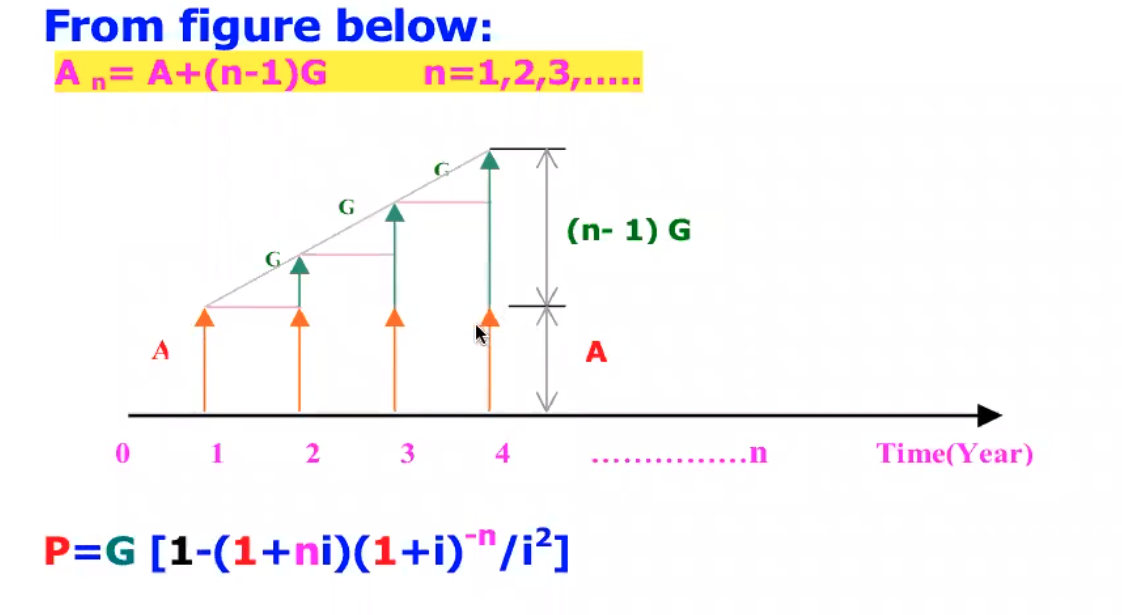
\includegraphics{/home/adrientremblay/Documents/school/summer 2020/ENGR 301/formulas/p1.png}

better formula using table vals

P=A(\(\frac{P}{A}\),i\%,n)+G(\(\frac{P}{G}\),i\%,n)

A=G(\(\frac{A}{A}\),i\%,n)+G(\(\frac{A}{G}\),i\%,n)

can also be A/G ??? for arithmetic gradient \emph{uniform} series

\hypertarget{geometric-gradient-series}{%
\section{Geometric Gradient Series}\label{geometric-gradient-series}}

\emph{If i != g}

P = \(A_{1}\frac{1-(1+g)^{n}(1+i)^{-n}}{i-g}\)

\emph{If i = g}

P = \(A_{1}\) {[}n ÷ (1 + i){]}

where:

\begin{itemize}
\tightlist
\item
  P is the present worth
\item
  r is the interest rate
\item
  g is the growth rate
\item
  n is the time period
\item
  \(A_{1}\) is the {[}initial{]} annual payment
\end{itemize}

\hypertarget{capitalized-cost}{%
\section{Capitalized Cost}\label{capitalized-cost}}

\textbf{Capitalized cost(P)} is the sum of money needed to forever
obtain exactly the payment amount needed(A) forever at a particular
interest rate(i).

\hypertarget{capital-recovery-formula-annual-cash-flow---salvage}{%
\section{Capital Recovery Formula (Annual Cash Flow -
Salvage)}\label{capital-recovery-formula-annual-cash-flow---salvage}}

\begin{itemize}
\tightlist
\item
  EUAC = P(A/P, i, n) -- S(A/F, i, n)
\end{itemize}

OR

\begin{itemize}
\tightlist
\item
  EUAC = (P -- S)(A/F, i, n) + Pi
\end{itemize}

OR

\begin{itemize}
\tightlist
\item
  EUAC = (P -- S)(A/P, i, n) + Si
\end{itemize}

\hypertarget{infinite-analysis}{%
\subsection{Infinite analysis}\label{infinite-analysis}}

P=A/i

(\(\frac{A}{P}\),i,infinity) = i

\hypertarget{present-worth-analysis-npwnet-present-value}{%
\section{Present Worth analysis NPW(Net Present
Value)}\label{present-worth-analysis-npwnet-present-value}}

NPW = the present value at t=0 lmao

\begin{itemize}
\tightlist
\item
  when doing NPW analysis we choose the plan with the \textbf{MAX} NPW
\item
  \textbf{ALWAYS} choose a GCM analysis period!
\end{itemize}

\hypertarget{annual-cash-flow-analysis}{%
\section{Annual cash flow analysis}\label{annual-cash-flow-analysis}}

\begin{itemize}
\tightlist
\item
  No need to find an equal analysis period
\end{itemize}

\hypertarget{rate-of-return-irr}{%
\section{Rate of Return (IRR)}\label{rate-of-return-irr}}

Interest rate when annual benefits are equivalent to annual cost.

\begin{itemize}
\tightlist
\item
  EUAB = EUAC
\end{itemize}

\emph{or}

Interest rate when PW = 0.

\begin{itemize}
\tightlist
\item
  If i gives a result to high go down and vice versa
\end{itemize}

\hypertarget{rate-of-returnirr-between-two-plans}{%
\subsection{Rate of Return(IRR) between two
plans}\label{rate-of-returnirr-between-two-plans}}

\begin{itemize}
\tightlist
\item
  Compute \(EUAB_{A-B}\) with an i to reach 0
\end{itemize}

\hypertarget{incremental-analysis}{%
\subsection{Incremental Analysis}\label{incremental-analysis}}

\begin{itemize}
\tightlist
\item
  Means of comparing different invenstements based on IRR.
\end{itemize}

For incremental IRR choose alternative with higher initial cost if IRR
\textgreater{} MARR

For \textbf{Aya's Method}:

\begin{itemize}
\tightlist
\item
  Order projects from left to right most expensive to least
\item
  start comparing pairs from the right
\item
  if the delta IRR is greater than MARR than the more expensive project
  is better and the losers should be elimenated
\item
  continue until there is a winner
\end{itemize}

\hypertarget{benefit-cost-ratio-analysis}{%
\section{Benefit-Cost Ratio
Analysis}\label{benefit-cost-ratio-analysis}}

EUAB/EUAC \textgreater{} 1 then accept otherwise reject

deltaEUAB/deltaEUAC \textless{} 1 then pick the trailer otherwise the
leader

\hypertarget{depreciation}{%
\section{Depreciation}\label{depreciation}}

\(BV_{t} = BV_{t-1} - D_{t}\)

\(D_{t} = BV_{t-1} - BV_{t}\)

\(BV_{t}=BV_{0} - \sum_{i=1}^{t} D_{t}\)

\hypertarget{straight-line-depreciation}{%
\subsection{Straight-Line
Depreciation}\label{straight-line-depreciation}}

\(d_{1} = (B-S)/N\)

where: * B is the \(BV_{0}\) * S is the salvage value * N is the useful
life of the asset

\hypertarget{sum-of-years-digits-depreciation-soyd}{%
\subsection{Sum Of Years Digits Depreciation
(SOYD)}\label{sum-of-years-digits-depreciation-soyd}}

\(d_{t}=\frac{N-t+1}{SOYD}(B-S)\)

where:

\begin{itemize}
\tightlist
\item
  \(d_{t}\) is the depreciation charge in any year t
\item
  N is the number of years in depreciable life
\item
  SOYD = N(N+1)/2 is sum of year's digits
\item
  B is the cost of the asset made ready for use
\item
  S is the estimated salvage value after depreciable life
\end{itemize}

\hypertarget{declining-balance}{%
\subsection{Declining Balance}\label{declining-balance}}

\hypertarget{normal-declining-balance}{%
\subsubsection{Normal Declining
Balance}\label{normal-declining-balance}}

\(BV_{t} = B(1-d)^{t}\)

\(d = 1-n\sqrt{\frac{S}{p}}\)

where:

\begin{itemize}
\tightlist
\item
  d is the depreciation \% rate
\item
  \textbf{that's an nth root buster}
\end{itemize}

\hypertarget{double-declining-balance}{%
\subsubsection{Double Declining
Balance}\label{double-declining-balance}}

\(d_{t}=(\frac{2}{N})(BV_{t-1})\)

where:

\begin{itemize}
\tightlist
\item
  BV is Book Value
\end{itemize}

\hypertarget{cca-capital-cost-allowance-rate}{%
\subsubsection{CCA (Capital Cost Allowance)
rate}\label{cca-capital-cost-allowance-rate}}

\(UCC_{t}=UCC_{t-1}-CCA_{t}\)

\(CCA_{t}=dUCC_{t-1}\)

\(UCC_{t}=B(1-d/2)(1-d)^{n-1}\)

\begin{itemize}
\tightlist
\item
  as long as n \textgreater{} 1
\end{itemize}

where:

\begin{itemize}
\tightlist
\item
  UCC is BV aka Book Value (CRA Terminology)
\item
  CCA is the depreciation amount
\item
  d is the depreciation rate
\end{itemize}

\textbf{Note:} You are only allowed to claim 50\% of your depreciation
on year 1!

\end{document}
